\chapter{前言}
\renewcommand{\baselinestretch}{10.0} %設定行距
\pagenumbering{arabic} %設定頁號阿拉伯數字
\setcounter{page}{1}  %設定頁數
\fontsize{14pt}{2.5pt}\sectionef

%-------------------研究動機與背景------------------------------%
\section{研究動機}
材料分析軟體的應用在機械領域愈來越廣泛,能夠將繪製零件進行分析,但卻鮮少人知道分析是怎麼進行的,所以我們對四足機器人套用有限元素法,在其身上觀察有限元素法是如何計算出受力情況。\\

本專題研究方向將由四足機器人(圖 \ref{四足機器狗(PLA)})作為載體,目的將有限元素分析的公式套入其中計算,進行有限元素分析,利用偏微分方程解出受力情況,才能對零件進行挖空處理,達到輕量化的目的,透過此過程從了解到運動模擬和有限元素法分析等。\\

\begin{figure}[hbt!]
\center
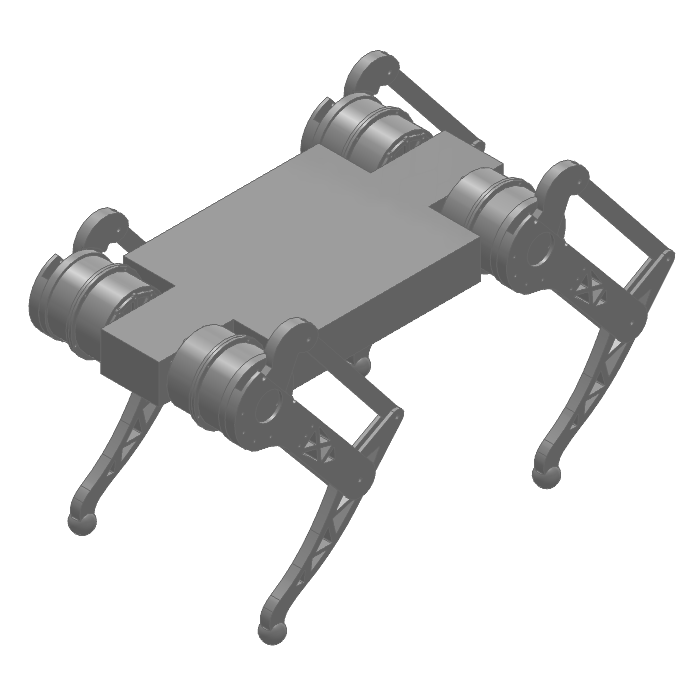
\includegraphics[width=10cm]{四足機器狗(PLA)}
\caption{\Large 虛擬四足機器人}\label{四足機器狗(PLA)}
\end{figure}
\newpage
%-----------------------研究目的--------------------------%
\section{研究目的及方法}
\begin{figure}[hbt!]
\begin{center}
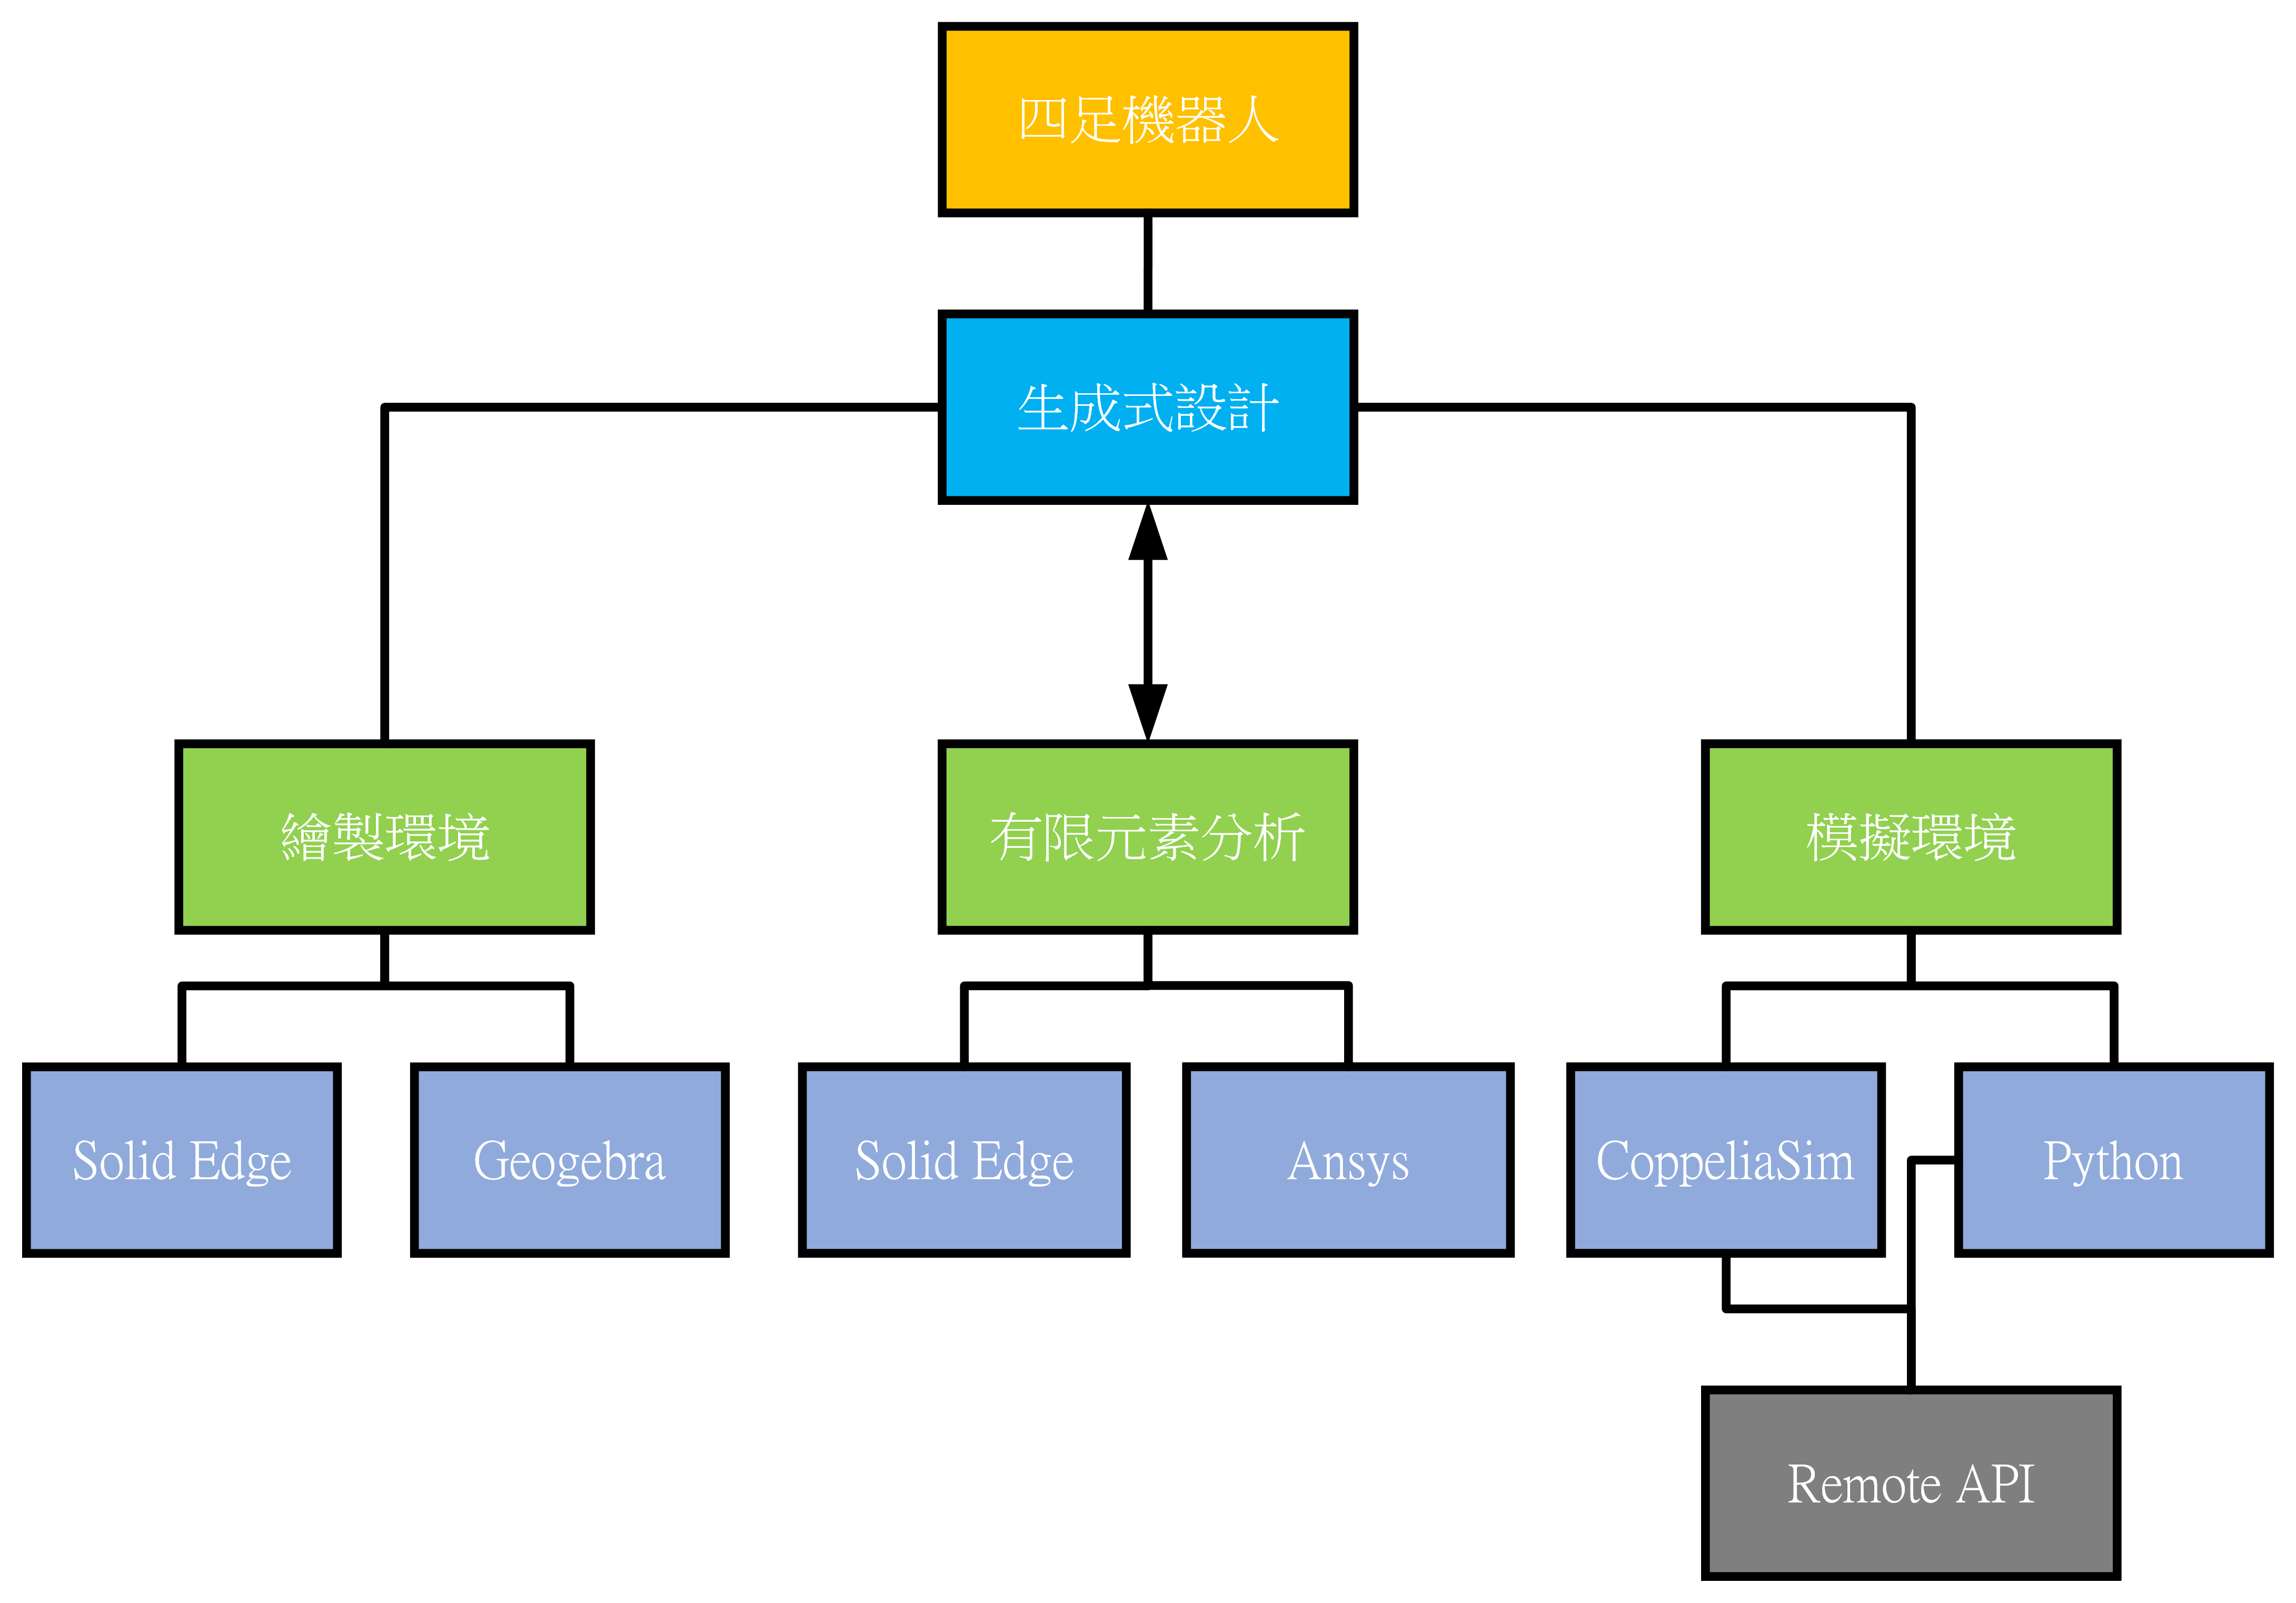
\includegraphics[width=13cm]{研究架構}
\caption{\Large 研究架構}\label{研究架構}
\end{center}
\end{figure}
本專題研究分為幾部分,其一繪製模型,進行路徑模擬,計算運動軌跡並調整設計,其二將模型導入虛擬環境進行運動模擬,找出運動姿態,其三為進行生成式設計,優化零件。\\

參考的四足機器人模型,將其利用繪製出模型並進行路徑分析,找出運動軌跡並用此調整連桿參數及推導運動學公式。\\

建立CoppeliaSim模擬環境,導入3D圖檔並組立進行結合,透過Python語言控制各步行機構作動及旋轉角度,以求得各零件最大受力情況,並結合Remote API對四足機器人進行遠端控制。\\

進行有限元素分析,透過上述過程即可得出受力狀況及3D模型,利用有限元素分析得知零件受力狀況,將可對其進行生成式設計,對零件非必要部分做挖空處理,減輕零件重量。\
\newpage
%----------------------分析說明------------------------%
\section{專題說明}
此專題主要研究有限元素法在四足機器人上的應用,模型部分參考了資料[1]及Goegebra路徑模擬,繪製出硬體架構,將其視為剛體帶入CoppeliaSim,由此可得知機器狗在機構為剛體狀態下的受力情況,。\\

對零件做有限元素分析,此狀態下的零件為柔性狀態會因為受力不同有變形情況,產生許多變量,像是位移、速度、加速度等,因此使用偏微分方程(PDE)對零件計算,進行離散化、代數方程導入、求解等步驟,此種方法稱為有限元素法。\\

比較兩軟體分析結果,進行生成式設計,進行四足機器人步行機構的輕量化處理,減輕零件重量並同時保有強度。\\

%----------------------文獻探討------------------------%
\section{文獻探討}

有限元素分析在設計領域運用得相當廣泛,在現今開發或製作幾乎成為必要的分析之一,對開發者而言,可以免去相當多的成本浪費,節省許多設計及修改時間,將目標模型直接進行分析得出受力情況,這些功能用來進行設計修正,也透過近來的AI機器學習的發展,誕生了生程式設計,給定參數就能利用AI迭代運算生成模型,不再受限於設計者的想像力。\\

近年來圍著機器人技術的發展,步行機器人的應用領域越來越廣,在軍用及工業等領域都可看見其身影,加上機械臂或其他工具,就可以勝任許多工作,漸漸替代傳統人力進行各式任務,進行高危或負重工作,因此我們將兩種結合,因為四足機器人在開發過程中通常會進行有限元素分析,主要用來做輕量化並找出最大負荷力,去除些許體積,在保有其性能的同時降低最多的能源消耗。\
\newpage

\renewcommand{\baselinestretch}{0.5} %設定行距
